\enteteThematiqueObligatoire{}
\enteteCorrection{}


%%%%%%%%%%%%%%%%%%%%%%%%%%%%%%%%%%%%%%%%%%%%%%%%%%%%%%%%%%%%%%%%%%
\encadreTDExo{1 - Boucle ouverte et boucle fermée}{
\begin{itemize}[label=$\triangleright$,leftmargin=*]
	\item Modélisation d'un Amplificateur Linéaire Linéaire - ordre 1
	\item Intérêt du rebouclage d'un ALI
\end{itemize}
}


%%%%%%%%%%%%%%%%%%%%%%%%%%%%%%%%%%%%%
\subsection*{Boucle ouverte et boucle fermée}

On s'intéresse au système bouclé suivant :

\begin{center}
	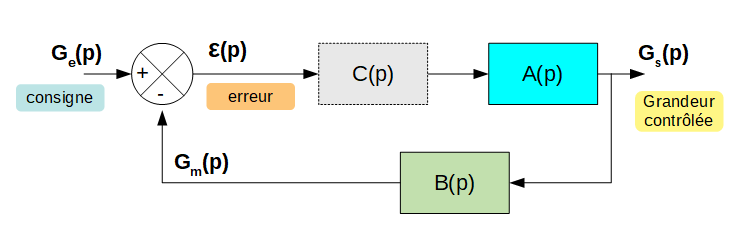
\includegraphics[width=13cm]{images/syst_asservi.png}
\end{center}

où :

\begin{itemize}
	\item $A(p)$ : système à asservir
	\item $B(p)$ : système de mesure (retour) de la grandeur à asservir
	\item $C(p)$ : correcteur de l'asservissement
	\item $G_e(p)$ : grandeur physique de consigne
	\item $G_s(p)$ : grandeur physique de sortie
	\item $\varepsilon(p)$ : erreur entre la consigne et la sortie
\end{itemize}


%%%%%%%%%%%%%%%%%%%%%%%%%%%%%%%%%%%%%
\subsection*{Boucle ouverte}

\begin{enumerate}
	\item Calculez la fonction de transfert en boucle ouverte : $TF_{BO}(p) = \frac{G_m(p)}{\varepsilon{}(p)}$
	\answer{
			$TF_{BO}(p) = \frac{G_m(p)}{\varepsilon{}(p)} = C(p) \cdot A(p) \cdot B(p)$
	}
	
	\item Calculez la fonction de transfert en boucle fermée, entre la consigne et la grandeur contrôlée : $TF_{BF}(p) = \frac{G_s(p)}{G_e(p)}$
	\answer{
			On a $G_s(p) = C(p) \cdot A(p) \cdot \varepsilon(p)$ et $\varepsilon(p) = G_e(p) - B(p) \cdot G_s(p)$
			
			On obtient alors : $G_s(p) = C(p) \cdot A(p) \cdot ( G_e(p) - B(p) \cdot G_s(p) )$
			
			Ce qui donne : $$TF_{BF}(p) = \frac{G_s(p)}{G_e(p)} = \frac{A(p) \cdot C(p)}{1 + A(p) \cdot C(p) \cdot B(p)} $$
	}
	
	\medskip 
	
	On notera $L(p) = A(p) \cdot B(p) \cdot C(p)$.
	
	\item Que devient l'expression précédente $TF_{BF}(p)$ ?
	\answer{
		$$TF_{BF}(p) = \frac{G_s(p)}{G_e(p)} = \frac{A(p) \cdot C(p)}{1 + L(p)} $$
	}

	\item Ce système peut-il être instable ?
	\answer{
			Il peut devenir instable si pour une valeur de fréquence (pulsation), $L(p) = -1$ (nombre réel de valeur égale à -1).
			
			Il existe des critères de stabilité basés sur les pôles de la fonction de transfert qui seront vus dans le cours d'automatique de 2A.
			
			\medskip
			
			\textbf{Début de démonstration}
			
			La réponse en fréquence d'un système peut se mettre sous la forme : $T_{FTBF}(p) = N(p) / D(p)$ où $N(p)$ et $D(p)$ sont des polynômes en $p$.
			
			Il est possible par décomposition en éléments simples d'obtenir la forme suivante : 
			
			$$T_{FTBF}(p) = \sum_k \frac{c_k}{p - a_k}$$
			
			où les $a_k$ sont réels ou complexes conjugués, ce sont les pôles de la fonction de transfert $T(p)$.

			Par fonction de Laplace inverse, on peut montrer que l'application d'un dirac sur un tel système amène la sortie à évoluer de la façon suivante :
			
			$$s(t) = \sum_k c_k \cdot e^{a_k \cdot t}$$
			
			Cette expression tend vers une valeur finie (amortissement) lorsque les \textbf{pôles $a_k$} de la fonction de transfert sont \textbf{à valeurs réelles négatives}. C'est une condition nécessaire à la stabilité d'un système.

	}
	\item Est-ce qu'un système d'ordre 1 stable (de la forme $A(p) = \frac{A_0}{1 + j\omega / \omega_0}$) non corrigé mais rebouclé peut devenir instable ? Un système d'ordre supérieur à 1 ?
	\answer{
		Dans le cas $A(p)$ du premier ordre, de la forme $A(p) = \frac{A_0}{1 + j\omega / \omega_0}$, par rebouclage, le dénominateur de la FTBF devient $1 + A(p) \cdot B(p)$. Le système reste stable si $B(p) = B_0 > 0$.
		
		\medskip
		
		Dans le cas $A(p)$ du second ordre, par rebouclage, le dénominateur de la FTBF peut devenir réel pur pour une valeur de fréquence particulière et avoir une valeur inférieure à -1. Dans ce cas, le système peut devenir instable.
		
		\medskip
			
		\textbf{Critères de stabilité}
		
		Selon le degré du polynôme $D(p)$, il peut être difficile d'en trouver les pôles.
		
		Il existe alors des critères (algébriques ou graphiques) permettant de déterminer la stabilité d'un système en boucle fermée à partir de l'étude en fréquence en boucle ouverte :
		
		\begin{itemize}
			\item \textbf{critère du revers de Nyquist} (basé sur l'étude dans le plan complexe de Nyquist) ;
			\item \textbf{critère de Routh}, critère permettant de déterminer à partir du polynôme $D(p)$ de la fonction de transfert le signe des racines de ce polynôme
		\end{itemize}
	}
\end{enumerate}

%%%%%%%%%%%%%%%%%%%%%%%%%%%%%%%%%%%%%
\subsection*{Boucle fermée}

En boucle fermée, on désire que le système :

\begin{itemize}
	\item suive la consigne en régime établi (précision)
	\item élimine les perturbations (rejet des perturbations)
	\item ait une dynamique rapide
\end{itemize}


%%%%%%%%%%%%%%%%%%%%%%%%%%%%%%%%%%%%%
\subsection*{Stabilité d'un système}

Certains systèmes bouclés peuvent devenir instable si la fonction de transfert en boucle ouverte s'approche trop près (pour certaines fréquences) de la valeur -1. En ajoutant des éléments correcteurs, il est possible de modifier le comportement et ainsi éviter que le système ne devienne instable, tout en essayant de le rendre plus rapide et plus robuste. 

Pour estimer les risques d'instabilité, on s'intéresse aux marges de gain et de phase d'un système en boucle ouverte, qui déterminera ensuite sa robustesse en boucle fermée.

Le point critique à ne pas franchir est le point -1, c'est à dire la pulsation pour laquelle $\lvert L(p) \rvert = 1 = 0dB$ et $arg(L(p)) = -\pi$.

On propose d'étudier le système dont on donne le diagramme de Bode suivant :

\begin{center}
	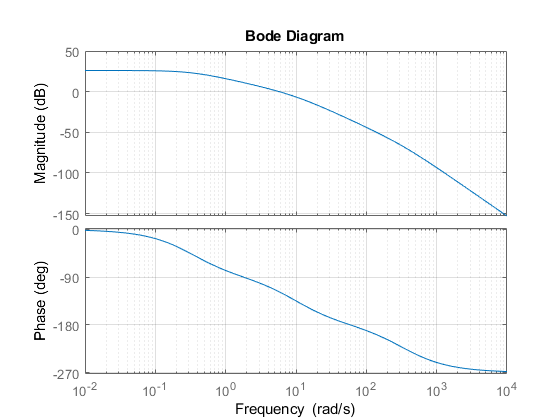
\includegraphics[width=15cm]{images/TD/sys_stable2.png}
\end{center}

\begin{enumerate}
	\item Mesurez les marges de gain et de phase et concluez sur sa stabilité en boucle fermée.

\answer{
\begin{center}
	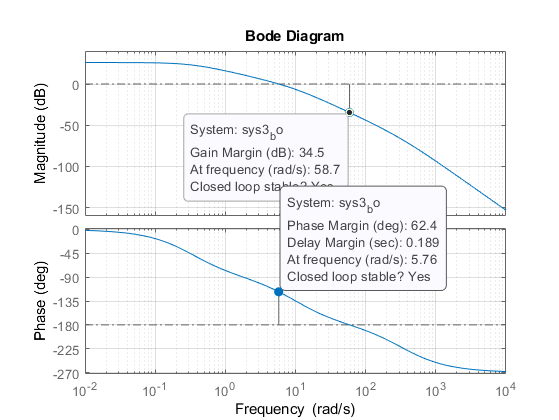
\includegraphics[width=13cm]{images/TD/sys_stable_corr.png}
\end{center}

Quelques informations sur ces marges :
\begin{itemize}
	\item \textbf{Un système est stable en BF si la marge de phase est positive}.
	\item La marge de gain correspond au gain supplémentaire maximum que l'on peut donner au système en BO sans risquer de le rendre instable en BF.
	\item Plus les marges sont grandes, plus robuste est la stabilité
\end{itemize}

}

	\item Qu'en est-il de ce nouveau système dont on donne le diagramme de Bode ?

\begin{center}
	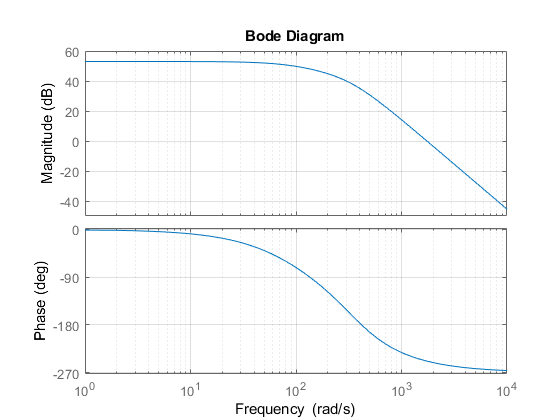
\includegraphics[width=15cm]{images/TD/sys_instable2.png}
\end{center}

\answer{
	Ce système est instable... Pour G = 0dB, on a une phase inférieure à -180$\deg{}$.
	
	La marge de phase est donc négative.
}

\end{enumerate}

%%%%%%%%%%%%%%%%%%%%%%%%%%%%%%%%%%%%%
\subsection*{Correction d'un système}

Dans cette partie, on utilisera comme exemple un système du premier ordre de la forme : 

$$H(p) = \frac{H_0}{1 + \tau \cdot p}$$

On prendra $H_0 = 0.5$ et $\tau = 2 \cdot 10^{-3}$

\begin{enumerate}
	\item Parmi les réponses en fréquence proposées par la suite, laquelle correspond :
\begin{enumerate}
	\item au système en boucle ouverte 
	\item au système en boucle fermée, avec un retour unitaire ($B(p) = 1$) et sans correction ($C(p) = 1$)
	\item au système en boucle fermée, avec un retour unitaire ($B(p) = 1$) et une correction proportionnelle ($C(p) = G$ avec $G = 10$)
	\item au système en boucle fermée, avec un retour unitaire ($B(p) = 1$) et une correction proportionnelle et intégrale ($C(p) = G + 1/(\tau_i \cdot p)$ avec $G = 10$ et $\tau_i = 3 \cdot 10^{-5}$)
\end{enumerate}

\begin{center}
	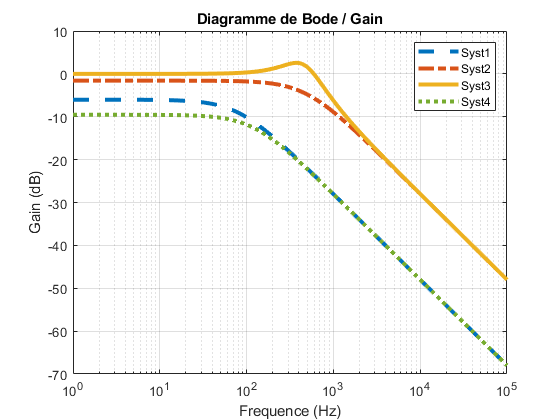
\includegraphics[width=15cm]{images/TD/sys_boucle_bode.png}
\end{center}

\answer{
	On peut calculer la fonction de transfert en boucle fermée, avec et sans correction.
	
	\textbf{Cas boucle fermé sans correction} (B = 1) : 
	$$FTBF(p) = \frac{H(p)}{1 + H(p)} = \frac{H_0}{1 + H_0} \cdot \frac{1}{1 + \frac{tau \cdot p}{1 + H_0}}$$
	
	Gain statique : $FTBF_0 = H_0 / (1 + H_0)$
	
	Constante de temps : $\tau_BF = \tau / (1 + H_0) < \tau$
	
	\textbf{Cas boucle fermé avec correction proportionnelle} (G = 10 et B = 1) : 
	$$FTBF(p) = \frac{C(p) \cdot H(p)}{1 + C(p) \cdot  H(p)} = \frac{G \cdot H_0}{1 + G \cdot H_0} \cdot \frac{1}{1 + \frac{tau \cdot p}{1 + G \cdot H_0}}$$	
	
	Gain statique : $FTBF_0 = G \cdot H_0 / (1 + G \cdot H_0) = 0.803 = -1.5\operatorname{dB}$
	
	Constante de temps : $\tau_BF = \tau / (1 + G \cdot H_0) < \tau$
	

	\textbf{Cas boucle fermé avec correction proportionnelle et intégrale} (G = 10 et B = 1) : 
	$$FTBF(p) = \frac{C(p) \cdot H(p)}{1 + C(p) \cdot  H(p)}$$	
	
	$$C(p) \cdot  H(p) = \frac{H_0 \cdot G \cdot \tau_i \cdot p + H_0}{\tau_i \cdot p + \tau \cdot \tau_i \cdot p}$$

	On obtient en boucle fermée une réponse du second ordre, qui peut être résonant.
	
	$$FTBF(p) = \frac{G \cdot \tau_i \cdot p}{1 + (1/H_0 + K) \cdot \tau_i \cdot p + \tau \cdot \tau_i p^2 / H_0}$$	
}
\answer{
	\textbf{Identification des réponses en fréquence} 

	Syst 1 : Sys Bouclé : on peut calculer le gain statique qui vaut $0.5/(1+0.5)$ ($G_0 = -9.6\operatorname{dB}$) et premier ordre

	Syst 2 : Sys Bouclé + P : erreur statique encore présente mais système plus rapide

	Syst 3 : Sys Bouclé + PI : pas d'erreur statique (gain statique = 0dB) et système avec la plus grande bande-passante, mais pouvant devenir très résonant

	Syst 4 : Sys Ouvert : $G_0 = -6\operatorname{dB}$ et premier ordre
	
	Il est intéressant de voir ici que le rebouclage et la correction d'un système permet de modifier sa réponse en fréquence et donc sa réponse à un échelon.
}

	\item Même question avec les réponses indicielles suivantes.

\begin{center}
	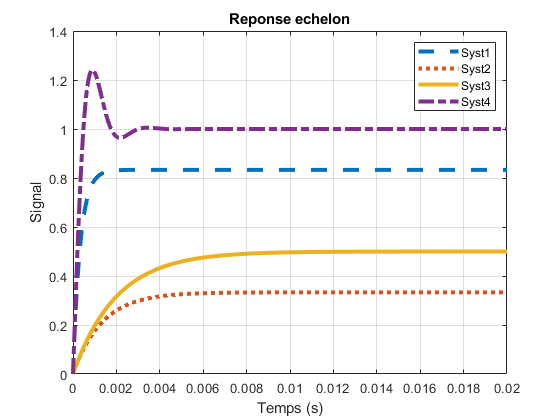
\includegraphics[width=15cm]{images/TD/sys_boucle_step.png}
\end{center}

\answer{
	Syst 1 : Sys Bouclé + P : erreur statique encore présente mais système plus rapide, mais pouvant devenir oscillant si G mal choisi

	Syst 2 : Sys Bouclé : on peut calculer le gain statique qui vaut $0.5/(1+0.5)$

	Syst 3 : Sys Ouvert : gain statique = 0.5 et constante de temps

	Syst 4 : Sys Bouclé + PI : pas d'erreur statique pour une consigne appliquée à 1 et résonance (ordre 2 à cause du correcteur)
	
	Il est intéressant de voir ici que le rebouclage et la correction d'un système permet de modifier sa réponse en fréquence et donc sa réponse à un échelon.
}

\seance{
On peut aussi introduire ici les lieux de Nyquist pour étudier ensuite la stabilité.

\begin{center}
	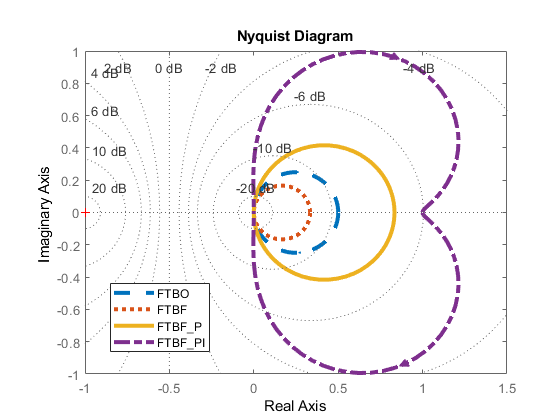
\includegraphics[width=12cm]{images/TD/sys_boucle_nyquist.png}
\end{center}

}

\end{enumerate}

%%%%%%%%%%%%%%%%%%%%%%%%%%%%%%%%%%%%%
\subsection*{Correction et stabilité}

On se base sur le système précédent, $H(p) = \frac{H_0}{1 + \tau \cdot p}$, rebouclé de manière unitaire ($B(p) = 1$) et une correction proportionnelle et intégrale ($C(p) = G + 1/(\tau_i \cdot p)$ avec $G = 10$).

Précisez si la correction intégrale est bien choisie dans les 4 cas suivants (réponse indicielle et réponse fréquentielle).

\begin{center}
	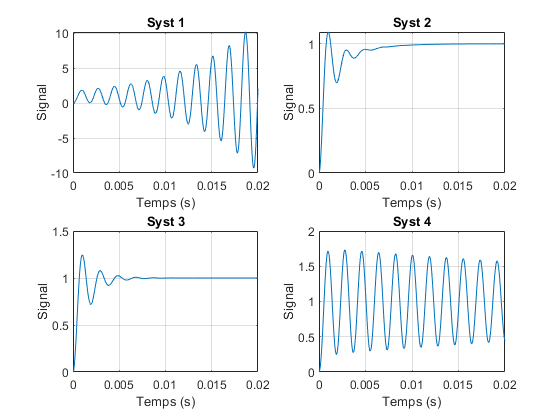
\includegraphics[width=8cm]{images/TD/sys_boucle_corrige_step.png} 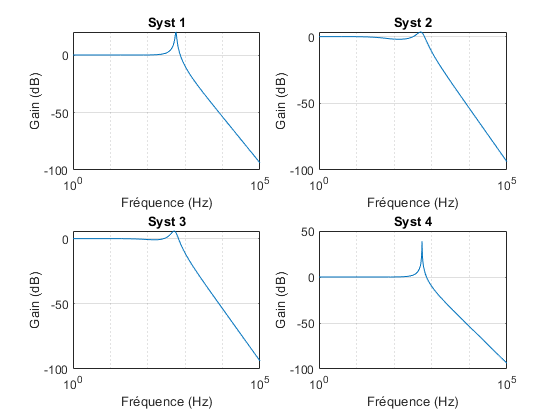
\includegraphics[width=8cm]{images/TD/sys_boucle_corrige_bode.png} 
\end{center}

\answer{
	Syst 1 : La réponse indicielle de ce système part à la dérive (ne converge pas). Ce système est instable.

	Syst 2 : La réponse indicielle de ce système est amortie, mais le temps de montée semble mal choisi. Le paramètre $\tau_i$ est probablement mal choisi.

	Syst 3 : La réponse indicielle de ce système est relativement bien amortie et tend vers une valeur finie. Le paramétrage du correcteur semble le meilleur dans ce cas là.

	Syst 4 : La réponse indicielle de ce système est peu amorti. Le correcteur semble mal paramétré.
}

%%%%%%%%%%%%%%%%%%%%%%%%%%%%%%%%%%%%%%%%%%%%%%%%%%%%%%%%%%%%%%%%%%
\encadreTDExo{2 - Exemple 1 : Amplificateur non-inverseur}{
\begin{itemize}[label=$\triangleright$,leftmargin=*]
	\item Système rebouclé basé sur les ALI
\end{itemize}
}

On rappelle qu'un ALI (Amplificateur Linéaire Intégré) peut être modélisé par une fonction de transfert du premier ordre du type : 

$$A(p) = \frac{A_0}{1 + \frac{p}{\omega_0}}$$

où $A_0$ est l'amplification différentielle statique et $\omega_0 = \frac{GBP}{A_0}$ la pulsation de coupure, avec $GBP$ la bande-passante unitaire.

On réalise autour de cet ALI un montage non-inverseur, dont le schéma est donné par la suite.

\begin{center}
	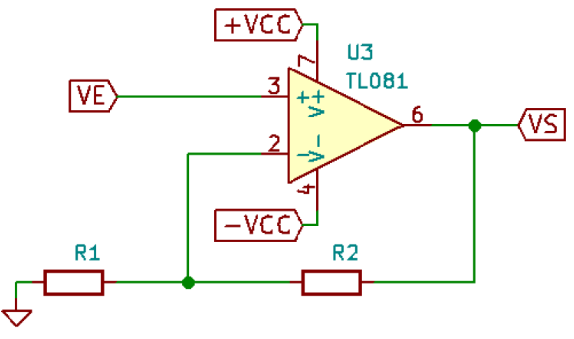
\includegraphics[width=10cm]{images/TD/noninverseur.png}
\end{center}

\begin{enumerate}
	\item Proposez un schéma bloc pour un \textbf{montage amplificateur non-inverseur}.
	\answer{
		\begin{center}
			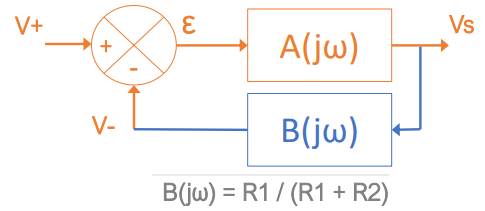
\includegraphics[width=8cm]{images/correction_ALI_BFnoninv.png}
		\end{center}
		
		$B(p) = V-(p) / V_S(p) = R_1 / (R_1 + R_2)$ si $R_2$ est la résistance de contre-réaction et $R_1$ la résistance à la masse.
	}
	
	\item Calculez la fonction de transfert en boucle fermée de ce montage. 
	\answer{
		On a $G(p) = A(p) / (1 + A(p) \cdot B(p)$ avec $A(p)$ la fonction de transfert de l'ALI et $B(p) = \frac{R_1}{R_1 + R_2}$.
		
		On obtient alors : 
		
		$$G(p) = \frac{\frac{A_0}{1 + \frac{p}{\omega_c}}}{1 + \frac{A_0}{1 + \frac{p}{\omega_c} \cdot \frac{R_1}{R_1 + R_2}}}$$
		
		Après simplification, on obtient : 
		
		$$G(p) = \frac{A_0}{1 + A_0 \cdot \frac{R_1}{R_1 + R_2}} \cdot \frac{1}{1 + \frac{p}{\omega_c} \cdot \frac{1}{1 + A_0 \cdot \frac{R_1}{R_1 + R_2}}}$$
	}
	\item Que valent à présent le gain statique et la pulsation caractéristique de ce système (pour les mêmes valeurs de $A_0$ et $GBP$) ?
	\answer{
		Le gain statique vaut alors : $G_0 = \frac{A_0}{1 + A_0 \cdot \frac{R_1}{R_1 + R_2}}$
		
		On peut simplifier si $A_0$ est "grand" par : $G_0 = \frac{R_1 + R_2}{R_1}$.
		
		La pulsation de coupure vaut : $\omega_0 = \omega_c \cdot (1 + A_0 \cdot \frac{R_1}{R_1 + R_2})$, 
				
		donc $f_0 = 2 \cdot \pi \cdot f_c \cdot (1 + A_0 \cdot \frac{R_1}{R_1 + R_2}) = GBP \cdot \frac{(1 + A_0 \cdot \frac{R_1}{R_1 + R_2})}{A_0}$.
		
		On peut là aussi simplifier si $A_0$ est "grand" par $f_0 = GBP \cdot \frac{R_1}{R_1 + R_2}$
	}	
\end{enumerate}


%%%%%%%%%%%%%%%%%%%%%%%%%%%%%%%%%%%%%%%%%%%%%%%%%%%%%%%%%%%%%%%%%%
\encadreTDExo{3 - Exemple 2 : Montage transimpédance}{
\begin{itemize}[label=$\triangleright$,leftmargin=*]
	\item Modélisation du montage transimpédance
\end{itemize}
}

On propose le montage transimpédance suivant :

\begin{figure}[!h]
\centering
\begin{circuitikz} 
	\node [op amp](A1) at (0,0){\texttt{ALI1}};
	\draw (A1.-) to[short] ++(-.5,0) coordinate(A) to[short] ++(0,1.5) coordinate(B) to[R=$R_F$, i=$i_R$] (B -| A1.out) to[short, -*] (A1.out);
	\draw (A1.- -| -5,0) node[ground]{};
	\draw (A1.- -| -5,0) to[I, invert, i=$i_{Phd}$, *-*] (A);
	\draw (A1.- -| -5,0) -- ++(0,1.5) to[C, l=$C_{Phd}$, i=$i_C$, -*] (B);
	\draw (A1.+) to[short] ++(0,-0.5) node[ground]{};
	\draw (A1.out) -- ++(1,0) coordinate(D);
	\draw (2.2,-2.1) edge[->, color={red}] (2.2,-0.3);
	\node[text={red}] (Vs) at (1.7,-1.2){$V_s$};
	\draw (2.2, -2.4) to[short, o-] ++(0,0.1) node[ground]{}; 
\end{circuitikz}
\end{figure}

On rappelle la fonction de transfert obtenue au TD précédent :

$$\frac{V_S}{i_{Phd}} = K \cdot \frac{R_F}{1 + p \cdot \frac{1}{1 + A_0} (\frac{\omega_c + \omega_0}{\omega_c \cdot \omega_0}) + (p)^2 \cdot \frac{1}{1 + A_0} \frac{1}{\omega_c \cdot \omega_0}}$$

où $\omega_0 = GBP / A_0$, $\omega_c = \frac{1}{R_F \cdot C_{Phd}}$ et $K = \frac{A_0}{1 + A_0}$

Il est possible de la mettre sous la forme d'un système rebouclé.

\begin{enumerate}
	\item Que valent alors les blocs $A(p)$ et $B(p)$ ?
\answer{
	$A(p)$ est la fonction de transfert de l'ALI de type : $A(p) = \frac{A_0}{1 + \frac{p}{\omega_0}}$
	
	Et $B(p)$ correspond à la fonction de transfert liée à $C_{Phd}$ et $R_F$.
	
	On peut aussi rappeler le schéma suivant pour le rebouclage :
	
\begin{center}
\begin{circuitikz}
	\draw (0,0) to[I,i=$i_{Phd}$,*-] (0,3) -- (2,3) -- (3,3) to[R,l=$R_F$, i=$i_R$] (5,3) to[short, -o] ++(0.5,0);
	\draw (0,0) -- (2,0) to[C,l=$C_{Phd}$,*-*, i=$i_C$] (2,3);
	\draw (2,0) -- (5,0) to[short, -o] ++(0.5,0);
	% fleches
	\draw (2.8,0.3) edge[->, green!40!black] (2.8,2.7); \node[text=green!40!black] (U-) at (3.2,1.5){$V-$};
	\draw (5.5,0.3) edge[->, red!40!black] (5.5,2.7); \node[text=red!40!black] (U-) at (5.9,1.5){$V_S$};
	\draw (0,0) node[ground](GND){};
\end{circuitikz}
\end{center}
}
	
	Dans un TD précédent, on obtient $V^- = (V_S + R_F \cdot i_{Phd}) \cdot \frac{1}{1 + p \cdot R_F \cdot C_{Phd}}$.
	
	On peut alors décomposer $V^-$ en deux parties :
	
	$V^-_1 = V_S \cdot \frac{1}{1 + p \cdot R_F \cdot C_{Phd}}$
	
	et 
	
	$V^-_2 = R_F \cdot i_{Phd} \cdot \frac{1}{1 + p \cdot R_F \cdot C_{Phd}}$
	
	
	On se retrouve alors avec le montage suivant :
	
	\begin{center}
		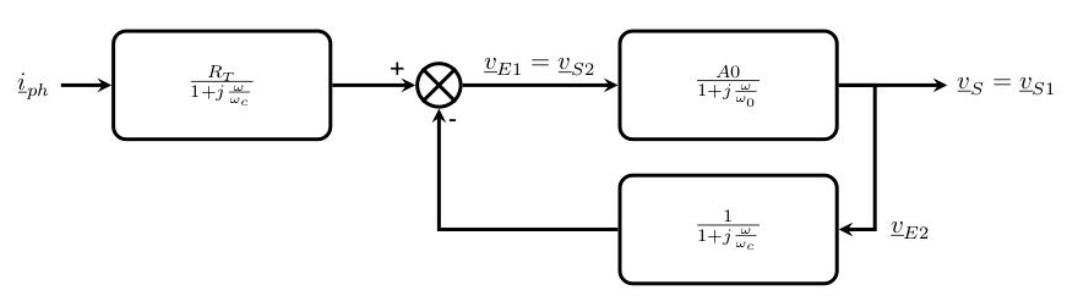
\includegraphics[width=14cm]{images/TD/trans_corr.png}
	\end{center}
	

	\medskip
	
	On rappelle que si on suppose $A_0 >> 1$, on obtient les valeurs de fréquence de coupure et de facteur d'amortissement suivantes :
	
		$$\omega_T \approx \sqrt{\omega_c \cdot A_0 \cdot \omega_0} = \sqrt{\omega_c \cdot \omega_{GBP}}$$
	
	$$m_T = \frac{\omega_c + \omega_0}{2 \cdot \omega_T} \approx \frac{1}{2} \cdot \sqrt{\frac{\omega_c}{\omega_{GBP}}}$$	
	

	\item Ce système peut-il devenir instable ?
	
\end{enumerate}